\section{AI-Assisted Authoring Workflow}
\label{sec:authoring-workflow}

Figure~\ref{fig:overall-architecture} shows the system architecture and an example flow.
The system is composed of two agents:

\begin{itemize}
    \item \textbf{SuggestionAgent}. LLM-based agent which identifies text fragments potentially computable from data.
    \item \textbf{InterpretationAgent}. LLM-based agent which, for a given text fragment (provided by
    SuggestionAgent or by the author), attempts to synthesise a Fluid expression computing the target text.
\end{itemize}

\begin{figure}
    \centering
    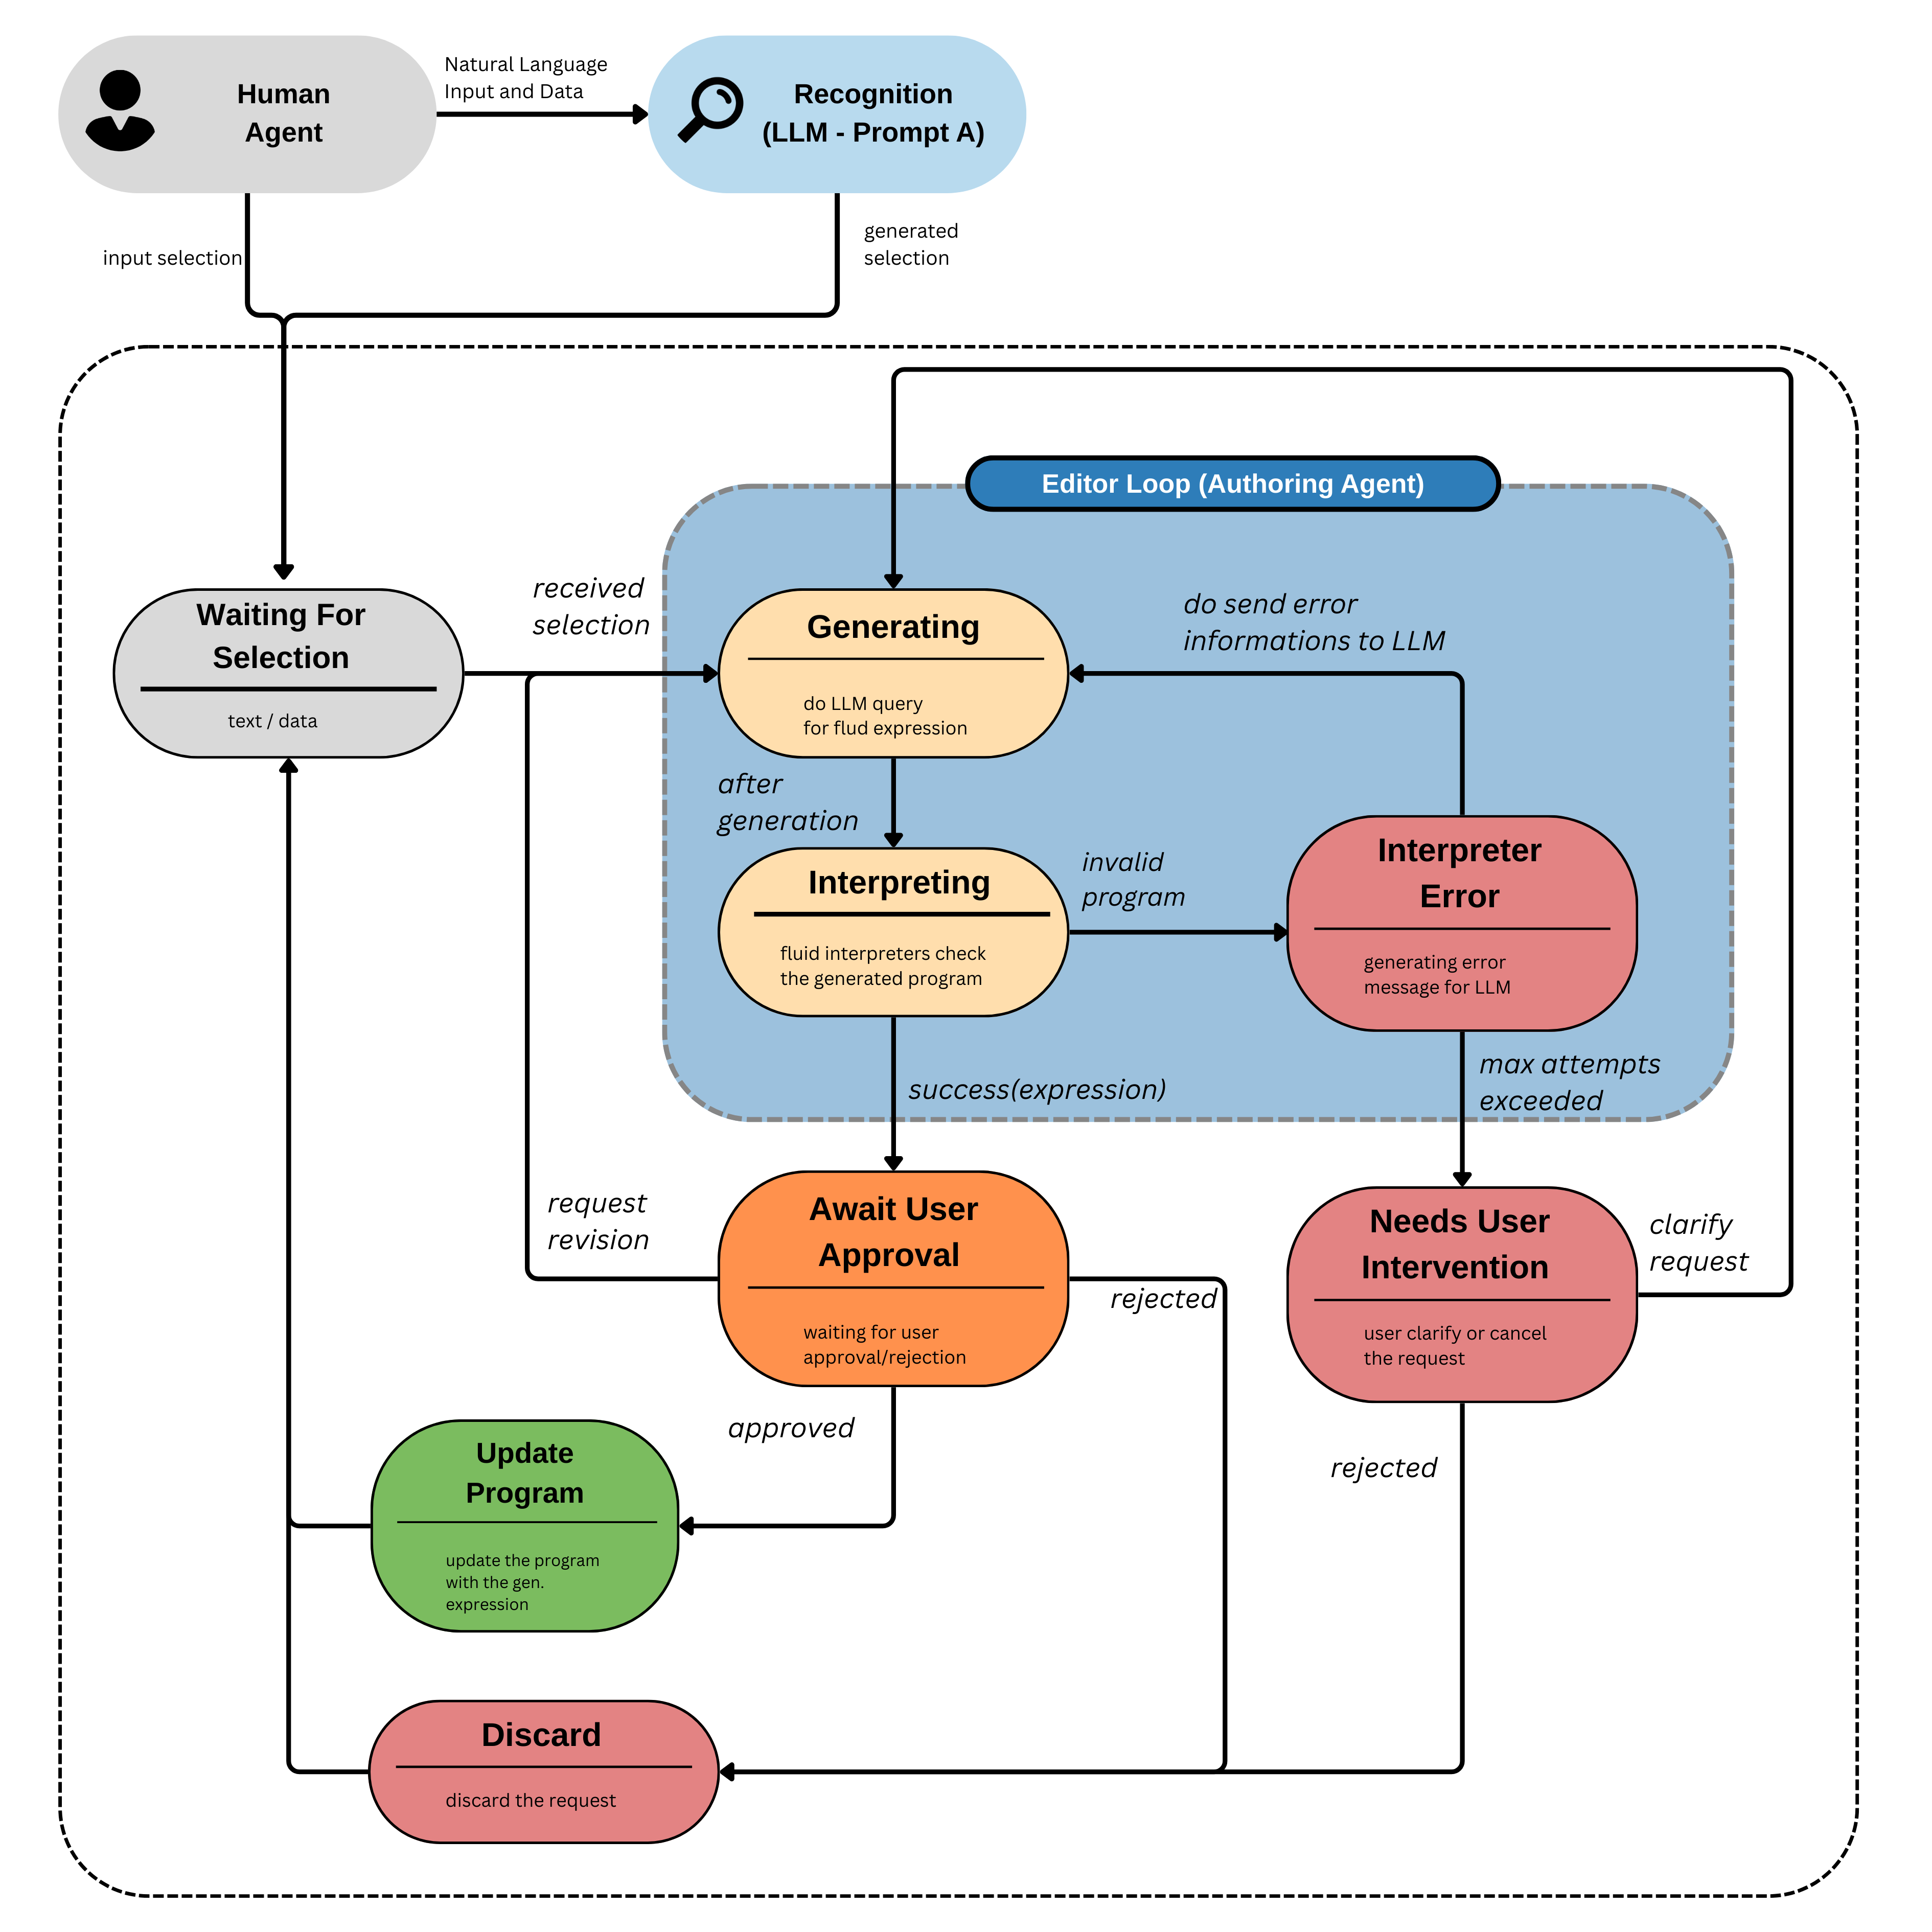
\includegraphics[width=\linewidth]{fig/entire-workflow}
    \caption{Workflow}\label{fig:architecture}
\end{figure}

Figure~\ref{fig:architecture} shows the overall architecture of the system.
The author initially provides the text and accompanying data.
The SuggestionAgent analyses the input and identifies candidate fragments of natural language which could be replaced by Fluid expressions.
The user highlightes a fragment of interest, which is then sent to the InterpretationAgent, which generates a corresponding candidate expression.
Internally the InterpretationAgent uses a compiler-in-the-loop validation process to ensure the expression is well-formed.
The user is then able to accept the expression (in which case it is incorporated into the program) or reject and leave the text uninterpreted.

\begin{figure}[ht]
    \centering
    \begin{subfigure}{0.50\linewidth}
        \centering
        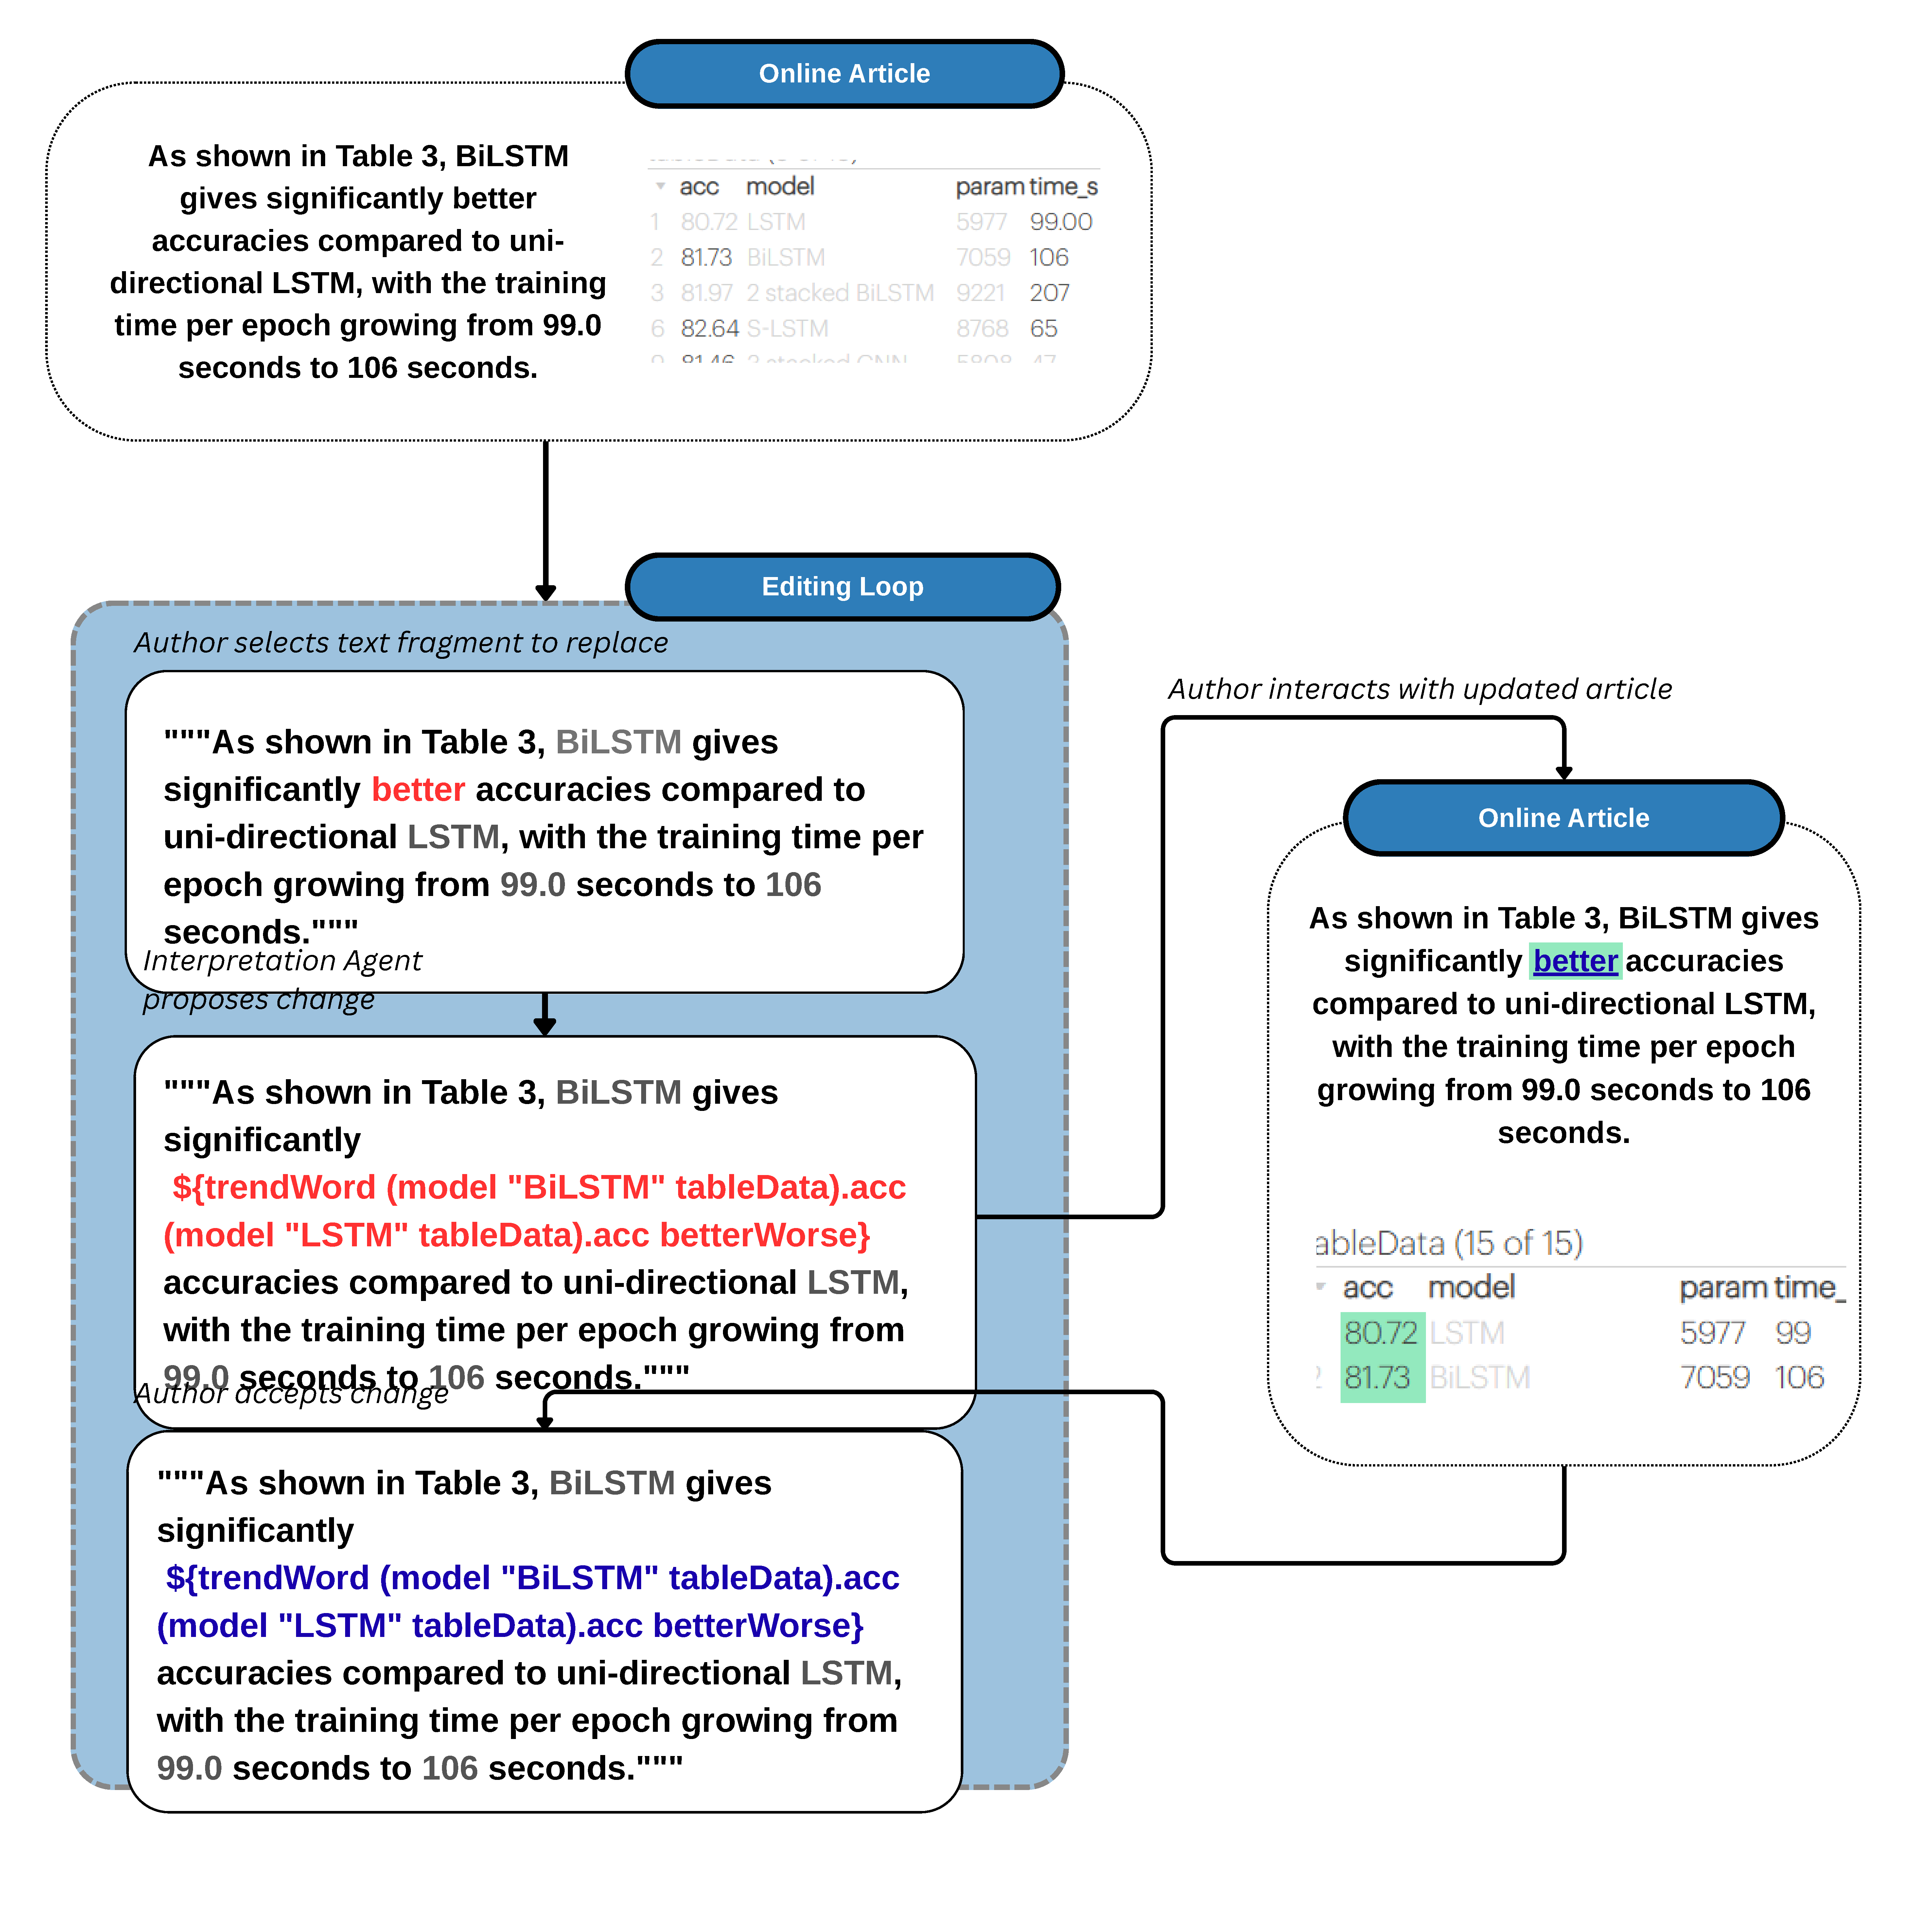
\includegraphics[width=\linewidth]{fig/data-flow-correct}
        \caption{Author Acceptance workflow}
        \label{fig:data-flow-correct}
    \end{subfigure}\hfill
    \begin{subfigure}{0.50\linewidth}
        \centering
        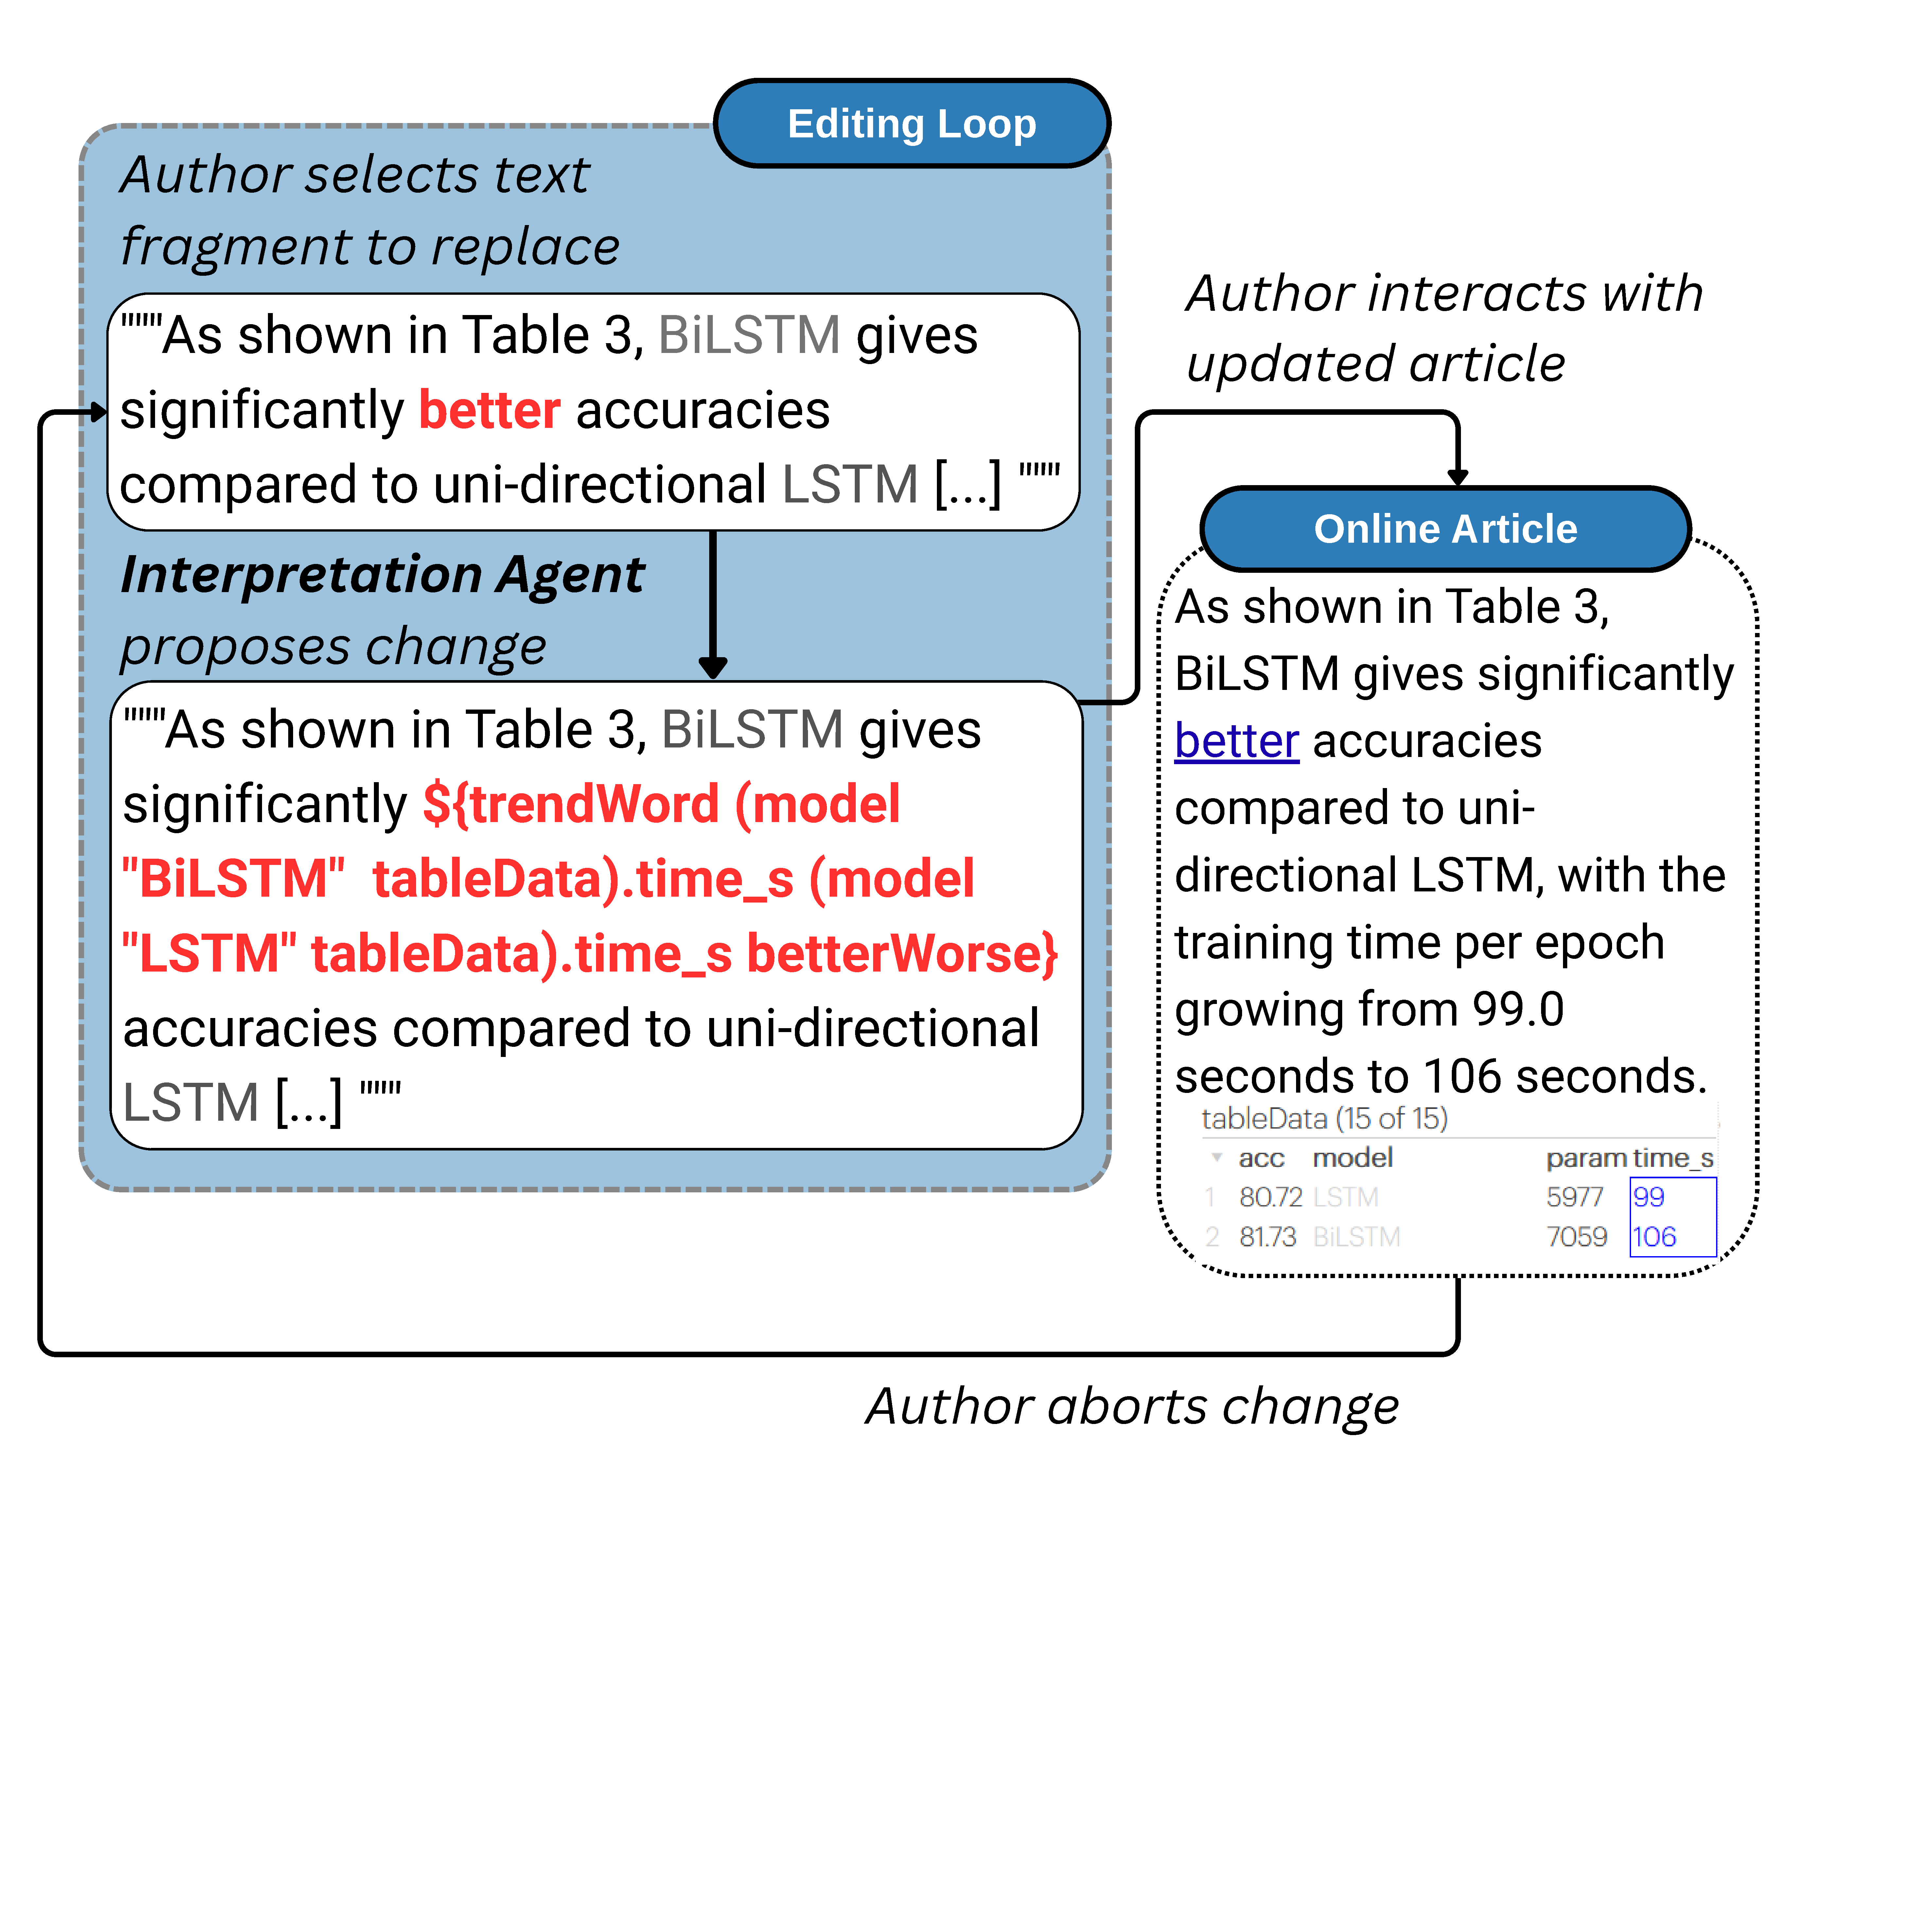
\includegraphics[width=\linewidth]{fig/data-flow-error}
        \caption{Author Rejection workflow}
        \label{fig:dataflow-error}
    \end{subfigure}
    \caption{Two possible paths through the basic editing loop: (a) author accepts generated expression after
    interactively verifying its correctness; (b) author rejects proposed expression, having identified an
    error (natural language mentions accuracy, while interaction reveals use of timing data).}
    \label{fig:overall-architecture}
\end{figure}


\subsection{System Prompt}
\label{subsec:system-prompt}
Fig. \ref{fig:system-prompt} shows the system prompt defined for the Authoring Assistant.

\begin{figure}[h]
    \centering
    \begin{tcolorbox}[colback=gray!10, colframe=gray!50, boxrule=0.5pt, arc=2pt,
        left=6pt, right=6pt, top=4pt, bottom=4pt]
        \VerbatimInput[fontsize=\small, formatcom=\normalfont]{../system-prompt/system-prompt.txt}
    \end{tcolorbox}
    \vspace{-0.5em}
    \caption{System Prompt defined for the Authoring Assistant}
    \label{fig:system-prompt}
\end{figure}


\subsection{Editor Loop}
\label{subsec:editor-loop}
Design of main loop that would be integrated into an IDE. The configuration (state) that is being maintained
is a \kw{Paragraph} the user is authoring in Fluid. Consists of a sequence of text fragments, some of which
are uninterpreted (plain literals), the remainder have underlying expressions linking the text to raw or derived
data.

Workflow:
\begin{enumerate}
\item User selects (a substring of) one of the literal text fragments, indicating they want to link it in this
way
\item Authoring tool generates expression which is either:
  \begin{enumerate}
  \item computes the selected text (e.g.~``greater than'' might be computed by comparing two numbers)
  \item becomes the formal meaning of the selected text (e.g. the text ``carbon intensity of methane
emissions'' can be understood in a specific context as referring to the numerical value ``34 gCO2eq/kWh''
  \end{enumerate}
\item Some kind of validation step, including both automated validation (e.g. checking for runtime errors) and
user validation; if validation fails, goto (2)
\item Partition code into additional definitions and expression; add definitions to main source file, and
incorporate expression into \kw{Paragraph}
\item Goto (1) with updated editor state
\end{enumerate}

\subsection{Loopback System}
\label{subsec:loopback-system}

Expressions generated by the \InterpretationAgent are evaluated by the Fluid interpreter. If evaluation fails,
the error is used to extend the prompt and the extended prompt is sent back to the LLM for regeneration. This
loopback mechanism enables iterative refinement of expressions, improving accuracy and robustness. There are
three kinds of loopback error:

\begin{itemize}
    \item \textbf{Invalid Program}. Evaluation fails due a syntax error, undeclared identifier, division by
    zero, array index out of bounds or other runtime problem.
    \item \textbf{Invalid Expression Type}. The value of the expression is not convertible to a string.
    \item \textbf{Mismatching String}. The string value of the expression is not equal to the target text.
\end{itemize}

\subsection{Paragraph with generated expression}
\label{subsec:paragraph-with-generated-expression}
Figure \ref{fig:fluid-example-paragraph} shows the Fluid code of a Paragraph with the expression generated by the authoring assistant.
Figure \ref{fig:fluid-scigen} shows the Fluid code written for the scigen datasets and examples.

\begin{figure}[h]
    \small
    {\lstinputlisting[language=Fluid]{../fluid-common/scigen.fld}}
    \caption{Fluid library written for scigen}
    \label{fig:fluid-scigen}
\end{figure}

\subsection{Turning validation errors into improved prompts}\label{subsec:turning-validation-errors-into-improved-prompts}
E.g.:
\begin{enumerate}
\item Turn ``Definition not found'' into prompt to generate definition?
\end{enumerate}

\subsection{IDE integration}\label{subsec:ide-integration}

Could then be integrated into desktop IDE like VSCode or online IDE like CodeMirror. Might make a good
internship project, but could also be out-of-scope for this paper.

\subsection{Other potential enhancements}\label{subsec:other-potential-enhancements}

We could also think about using an LLM in a couple of other complementary ways:
\begin{itemize}
\item identifying text fragments which might be linked;
\item validating generated expressions (perhaps by proposing test cases)
\end{itemize}


